\documentclass[11pt]{article}

\usepackage[margin=0.86in]{geometry}
\usepackage{amsmath}
\usepackage{amssymb}
\usepackage{booktabs}
\usepackage{graphicx}
\usepackage{microtype}
\usepackage{array}
\usepackage{longtable}
\usepackage{float}
\usepackage{url}
\usepackage{xcolor}
\usepackage[hidelinks]{hyperref}

\definecolor{resultblue}{HTML}{2563EB}
\definecolor{warningorange}{HTML}{B45309}
\definecolor{passgreen}{HTML}{047857}
\definecolor{failred}{HTML}{B91C1C}
\newcommand{\pass}{\textcolor{passgreen}{\textbf{PASS}}}
\newcommand{\fail}{\textcolor{failred}{\textbf{FAIL}}}
\newcommand{\code}[1]{\texttt{#1}}

\title{\textbf{Typed Neural Firmware versus a Learned-Parser
IGC-Style Calculator in Qwen2.5-0.5B}\\
\large A Frozen Three-Seed, Same-Prompt Comparison of Reliability,
Parameter Efficiency, and Preservation}
\author{Josiah Wilson\\Independent Researcher}
\date{July 26, 2026}

\begin{document}
\maketitle

\begin{abstract}
We compare two ways to install exact addition inside the same frozen
Qwen2.5-0.5B-Instruct model. \emph{Typed neural firmware} receives two
decimal operands from a fixed character boundary, uses a learned semantic
router, executes a frozen ripple-carry process, and returns the result through
a learned residual codebook. An independent \emph{IGC-style} architecture
learns operand registers directly from early model residuals, routes from a
late residual, applies the same class of frozen calculator, and uses a learned
gated output mapping. We trained three paired seeds and evaluated an untouched
base, an ordinary learned adapter, typed firmware, an exactly
parameter-matched IGC-style model, and a native-size IGC-style model on the
same 400 held-out natural-language addition prompts and 160 adversarial
non-addition prompts per seed.

Typed firmware was correct on 1,200/1,200 addition predictions (100\%) using
24,225 learned parameters. Native IGC-style was correct on 1,084/1,200
(90.33\%) using 597,819 learned parameters; its seed accuracies were 96\%,
85\%, and 90\%. Typed minus native accuracy was +9.67 percentage points, with
a precommitted paired crossed seed/prompt bootstrap 95\% interval of +4.33 to
+15.25 points. The native model recovered both operand registers on
1,083/1,200 prompts and was correct on all 1,083 of those cases, localizing
its errors to learned extraction. The exactly matched 24,225-parameter
IGC-style model recovered zero complete registers and scored 1/1,200; the
ordinary adapter scored 33/1,200.

The frozen ``comparably reliable'' equivalence rule failed because the
typed--native interval was not contained within $\pm5$ points; typed was more
accurate, not equivalent. The parameter-efficiency rule passed: typed was not
less accurate, used 24.68 times fewer learned parameters, and matched native
preservation. However, both models falsely routed 18/480 multiplication
prompts and preserved only 462/480 negative outputs token-for-token (96.25\%),
missing the preregistered 2\% false-route and 99\% preservation gates. The
result therefore supports a reliability and parameter-efficiency advantage
for typed firmware \emph{when a fixed parser is allowed}, while exposing
operation routing and learned extraction as the remaining bottlenecks. It is
an independent IGC-style comparison, not a reproduction of Dietz and Klakow's
larger four-operation system.
\end{abstract}

\section*{Technical summary}

\begin{center}
\small
\begin{tabular}{p{0.32\linewidth}rrr}
\toprule
Condition & Learned parameters & Correct & Accuracy\\
\midrule
Untouched base & 0 & 68/400 & 17.0\%\\
Ordinary adapter & 24,225 & 33/1,200 & 2.75\%\\
Typed firmware & 24,225 & 1,200/1,200 & 100.0\%\\
Matched IGC-style & 24,225 & 1/1,200 & 0.083\%\\
Native IGC-style & 597,819 & 1,084/1,200 & 90.33\%\\
\bottomrule
\end{tabular}
\end{center}

\noindent\textbf{Primary result.}
Typed firmware produced no arithmetic or format error in three seeds and
outperformed the native learned-parser comparator by 9.67 points. Native IGC
was conditionally exact after successful operand extraction, but register
accuracy varied materially by seed.

\medskip
\noindent\textbf{Frozen interpretation.}
The symmetric equivalence criterion is a \fail: its full confidence interval
did not fall within -5 to +5 points. The parameter-efficiency criterion is a
\pass: typed used only 4.05\% as many learned parameters, was more accurate,
and had equal preservation.

\medskip
\noindent\textbf{Safety verdict.}
Arithmetic reliability did not imply safe invocation. All trained conditions
exceeded the fixed 2\% false-route maximum and missed 99\% token preservation.
The router consistently mistook one held-out multiplication wording for
addition.

\medskip
\noindent\textbf{Claim boundary.}
Typed firmware uses a fixed parser; native IGC learns its operands. The
comparison answers how the complete architectures perform on identical
prompts, but it does not show that typed firmware learned parsing with fewer
parameters. The matched-budget IGC failure is specific to the selected mapper
and allocation, not an impossibility theorem.

\section{Motivation and closest prior work}

Exact arithmetic combines a flexible language-interface problem with a rigid
state-transition problem. Neural models can learn correlations over arithmetic
strings but often generalize poorly beyond trained lengths or distributions
\cite{trask2018,jelassi2023,cho2024}. Algorithmic modules and compiled
transformer programs instead encode known transitions structurally
\cite{lindner2023,bounsi2024}.

The closest prior work is Dietz and Klakow's Integrated Gated Calculator
(IGC) \cite{dietz2025}. Their system freezes Llama 3.1 8B and learns an
approximately 17-million-parameter module containing a categorical
number/operator input mapping, a gate, a non-differentiable calculator, and an
output mapping. The module executes within a model forward iteration and
reports 98--99\% on four arithmetic operations. That work establishes direct
prior art for the broad concept of a learned internal interface around an
exact calculator.

Earlier phases of the present project installed a frozen typed ripple-carry
process in small trained transformers and then inside frozen
Qwen2.5-0.5B-Instruct \cite{qwen2024}. Phase 4 used a fixed two-number parser
and learned natural-language router. It reached 90\% on 400 prompts and 100\%
with routing forced on, but did not directly compare with a learned input
mapping.

Phase 5 addresses that missing comparison:

\begin{quote}
On one frozen small model, identical training data, identical held-out
addition prompts, and identical adversarial negatives, does typed neural
firmware offer a reliability or parameter-efficiency advantage over an
IGC-style learned input/calculator/output architecture?
\end{quote}

This is not a reproduction of the original IGC result. Its code was
unavailable, and the present model, task scope, prompt distribution,
optimization, and module sizes differ. ``IGC-style'' denotes the shared
functional decomposition and auxiliary categorical input supervision.

\section{Architecture}

\subsection{Frozen base}

Every condition uses
\code{Qwen/Qwen2.5-0.5B-Instruct}, revision
\code{7ae557604adf67be50417f59c2c2f167def9a775}. Its 494,032,768 pretrained
parameters remain frozen. Generation uses the same chat template, greedy
decoding, and token budgets. The untouched base is evaluated once rather than
duplicated to create artificial replication.

\subsection{Typed neural firmware}

The typed condition retains the Phase 4 decomposition:
\[
\text{fixed decimal boundary}
\rightarrow
\text{learned semantic router}
\rightarrow
\text{frozen ripple-carry addition}
\rightarrow
\text{learned residual codebook}.
\]

The boundary identifies exactly two contiguous nonnegative decimal strings
and converts them to typed digit registers. It does not choose the operation.
A width-16 router observes the final request residual after transformer block
24 and before final RMS normalization. If active, a zero-parameter
ripple-carry cell emits one of eleven symbols (digits 0--9 or end), and a
learned codebook drives the frozen output head. The router contains 14,369
parameters and the output codebook 9,856, for 24,225 total.

\subsection{Ordinary learned adapter}

The adapter shares the same 14,369-parameter late router and replaces the
typed cell/codebook with a rank-five SiLU residual adapter containing 9,856
parameters. It receives no operands or deterministic state. Its 24,225 total
parameters exactly match typed firmware.

\subsection{Dual-depth IGC-style architecture}

The IGC-style conditions receive no parsed operands at inference. After block
1, a learned bidirectional sequence encoder processes token residuals. Two
sets of learned anchor queries attend to the sequence and predict twelve
least-significant-digit-first slots per operand, each categorical over digits
0--9 and PAD. Training provides auxiliary digit/PAD targets. Argmax registers
feed the frozen calculator.

Semantic routing and output are deliberately placed later. A block-24 router
chooses addition/no-operation. When active, a learned gated output mapping
translates calculator symbols into the block-24 residual stream. This
dual-depth design was selected on development data because early residuals
preserved digit identity while late residuals separated request intent.

The matched variant allocates:

\begin{center}
\small
\begin{tabular}{lr}
\toprule
Component & Learned parameters\\
\midrule
Input mapper & 16,986\\
Linear late router & 897\\
Gated output mapping & 6,342\\
\midrule
Total & 24,225\\
\bottomrule
\end{tabular}
\end{center}

Its bidirectional encoder has only three units per direction. This was the
best exact-budget allocation found in pilot work, but recovered no complete
development registers.

The native variant uses 64 units per direction, eight attention heads, a
width-16 late router, and a full output codebook:

\begin{center}
\small
\begin{tabular}{lr}
\toprule
Component & Learned parameters\\
\midrule
Input mapper & 572,696\\
Late router & 14,369\\
Gated output mapping & 10,754\\
\midrule
Total & 597,819\\
\bottomrule
\end{tabular}
\end{center}

\section{Pilot development and frozen protocol}

\subsection{Mapper selection}

Direct linear and feed-forward anchor mappers failed to maintain Qwen's
grouped-number token order. Initial exact-register accuracy was 3.5\% for the
matched allocation and 9.5\% for an early native allocation. A bidirectional
sequence encoder raised native block-1 recovery to 78\%; separating early
extraction from late routing/output raised a dual-depth pilot to 93.5\%.
The matched mapper remained at zero complete registers after budget
reallocation. Those failed pilots and their compact result files were retained.

\subsection{Feature-point correction}

The first three-seed training pass collected late router features from
\code{hidden\_states[24]}, which Qwen returns after final RMS normalization.
Installed wrappers instead see the block-24 residual before that
normalization. A direct hook measured norms of 46.33 versus 254.05 and a
maximum coordinate difference of 86.65. Before any confirmatory inference,
routers were recalibrated on the correct pre-normalization residual; all
superseded checkpoints were retained.

The resulting native development-register accuracies were 97.125\%, 94.750\%,
and 89.500\% across seeds. An integrated 10-positive/20-negative diagnostic
per seed yielded 30/30 typed and 28/30 native positive answers, 60/60 positive
routes, and no false routes. Only then was the protocol frozen.

\subsection{Training and seeds}

Seeds 10,701, 10,702, and 10,703 use the same deterministic data generator and
optimization counts. Training contains 2,400 positive and 2,400 negative
routing/input examples with one- through twelve-digit operands, 1,600
positive output/adapter examples with one- through eight-digit operands, and
800 development examples. IGC input training uses supervised digit/PAD and
operation targets. Output training uses the ground-truth calculator result
before free-running evaluation.

\subsection{Confirmatory prompts}

The frozen confirmation contains four 100-prompt positive splits:

\begin{enumerate}
  \item unseen simple wording, one- through four-digit operands;
  \item unseen simple wording, five- through eight-digit operands;
  \item unseen simple wording, nine- through twelve-digit operands;
  \item unseen word problems, five- through eight-digit operands.
\end{enumerate}

The 160 negative prompts cover subtraction, multiplication, division,
remainder, comparison, concatenation, repetition, quotation, refusal,
explanation, parity-like requests, syntax, identifiers, and averaging. Every
condition receives the exact same rendered prompts in the same order. Raw
text, token IDs, route scores, register predictions, correctness, and latency
are retained.

\subsection{Outcomes and inference}

The primary endpoint is mathematical correctness: the last decimal integer in
the response must equal the exact sum. Exact-format correctness is secondary.
Other outcomes are route recall, false-route rate, token-exact preservation
against base, operand-register recovery, arithmetic conditional on correct
routing/registers, latency, and learned parameters.

Paired accuracy differences use a 20,000-draw bootstrap that independently
resamples the three paired training-seed clusters and 400 paired prompt
clusters. Exact McNemar tests are reported separately by seed; pooled
discordant counts are descriptive because prompts repeat across seeds. Wilson
intervals describe binomial routing, preservation, and register rates.

The architectures are ``comparably reliable'' only if the entire 95\%
interval for typed minus native accuracy is contained in $[-5,+5]$ percentage
points. Typed has a parameter-efficiency advantage if it is no more than five
points below native, uses at most one tenth as many learned parameters, and
has preservation no more than one point below native. Operational routing
requires at least 90\% positive recall and at most 2\% false activation;
preservation requires at least 99\% token identity.

\section{Results}

\subsection{Arithmetic accuracy}

\begin{figure}[H]
\centering

\includegraphics[width=0.86\linewidth]{figures/aggregate_accuracy.pdf}
\caption{Confirmatory mathematical accuracy. Trained-condition bars are means
over three seeds and 400 prompts per seed; the untouched base is evaluated
once on 400 prompts.}
\label{fig:aggregate}
\end{figure}

Typed firmware answered all 1,200 prompts mathematically and format exactly.
The ordinary adapter produced 33 mathematical successes and 32 exact-format
successes. Matched IGC produced one success. Native IGC produced 1,084
mathematical and exact-format successes.

\begin{table}[H]
\centering
\small
\begin{tabular}{lrrrr}
\toprule
Condition & Seed 10,701 & Seed 10,702 & Seed 10,703 & Pooled\\
\midrule
Adapter & 13/400 & 10/400 & 10/400 & 33/1,200\\
Typed firmware & 400/400 & 400/400 & 400/400 & 1,200/1,200\\
Matched IGC & 0/400 & 0/400 & 1/400 & 1/1,200\\
Native IGC & 384/400 & 340/400 & 360/400 & 1,084/1,200\\
\bottomrule
\end{tabular}
\caption{Per-seed mathematical correctness.}
\label{tab:seed-accuracy}
\end{table}

The native seed standard deviation was 5.51 percentage points. Typed firmware
had zero observed between-seed variation. By split, native seed-mean
accuracies were 94.33\% for one--four digits, 89.67\% for five--eight digits,
90.0\% for nine--twelve digits, and 87.33\% for word problems. The word split
was least stable, ranging from 74\% to 100\%. Typed scored 100\% on each split
and seed.

\begin{figure}[H]
\centering

\includegraphics[width=0.92\linewidth]{figures/accuracy_by_split.pdf}
\caption{Accuracy by frozen positive split. Typed and native values are
three-seed means; base is the single untouched run.}
\label{fig:splits}
\end{figure}

\subsection{Paired comparisons and frozen decisions}

\begin{table}[H]
\centering
\small
\begin{tabular}{lrr}
\toprule
Typed comparison & Difference (pp) & Crossed bootstrap 95\% interval\\
\midrule
versus untouched base & +83.00 & [+79.25, +86.75]\\
versus ordinary adapter & +97.25 & [+95.67, +98.67]\\
versus matched IGC & +99.92 & [+99.58, +100.00]\\
versus native IGC & +9.67 & [+4.33, +15.25]\\
\bottomrule
\end{tabular}
\caption{Paired mathematical-accuracy differences. The base result is
repeated only as the paired comparator within each seed; the bootstrap
clusters the repeated prompts and seeds.}
\label{tab:paired}
\end{table}

For typed versus native, per-seed discordant pairs were 16--0, 60--0, and
40--0 in typed's favor. Exact McNemar $p$-values were
$3.05\times10^{-5}$, $1.73\times10^{-18}$, and
$1.82\times10^{-12}$, respectively. No comparator was correct where typed
was wrong.

The equivalence decision is \fail{} because the upper confidence limit exceeds
+5 points. This wording matters: the failure is not evidence of worse typed
reliability. It indicates that the observed typed advantage is too large to
call the systems equivalent under the frozen rule.

The parameter-efficiency decision is \pass{}. Typed is more accurate, has
identical preservation, and uses 24.68 times fewer learned parameters.
Figure~\ref{fig:parameters} visualizes the architectural tradeoff.

\begin{figure}[H]
\centering
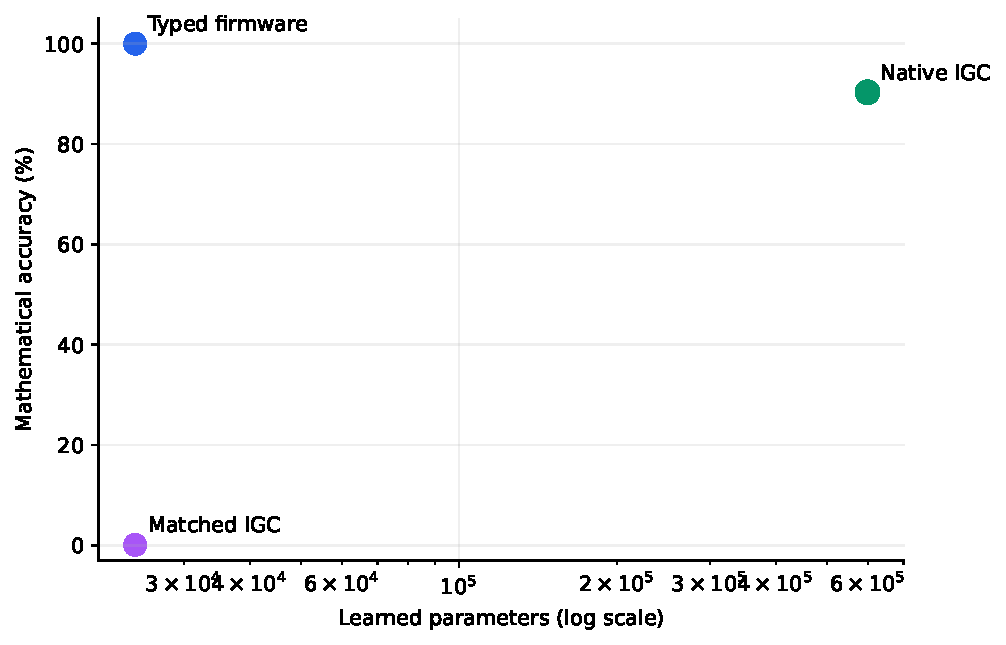
\includegraphics[width=0.76\linewidth]{figures/accuracy_vs_parameters.pdf}
\caption{Seed-mean mathematical accuracy versus learned interface parameters.
The shared $x$ coordinate for typed and matched IGC reflects their exact
24,225-parameter match.}
\label{fig:parameters}
\end{figure}

\subsection{Operand extraction localizes native IGC errors}

Native exact-register recovery was 384/400, 340/400, and 359/400 across seeds,
or 1,083/1,200 pooled. All 1,083 prompts with route and both registers correct
produced the exact sum. One seed-10,703 prompt produced the correct final
answer despite an incorrect register, yielding 1,084 total successes.

Matched IGC recovered no exact operand pair. Its recurrent width of three per
direction was insufficient for the selected twelve-slot mapping. Because the
calculator never received the right complete state, the matched result does
not diagnose calculator execution.

These observations provide a useful stage decomposition:
\[
\underbrace{\text{route}}_{100\%\ \text{positive recall}}
\quad+\quad
\underbrace{\text{extract}}_{90.25\%\ \text{native registers}}
\quad+\quad
\underbrace{\text{execute/output}}_{100\%\ \text{when eligible}}.
\]
Native end-to-end reliability is limited by extraction. Typed firmware
eliminates that learned stage through its fixed boundary.

\subsection{Routing and preservation}

\begin{table}[H]
\centering
\small
\begin{tabular}{lrrr}
\toprule
Condition & Positive routes & Negative false routes & Token preserved\\
\midrule
Adapter & 1,200/1,200 & 18/480 (3.75\%) & 468/480 (97.5\%)\\
Typed firmware & 1,200/1,200 & 18/480 (3.75\%) & 462/480 (96.25\%)\\
Matched IGC & 1,200/1,200 & 24/480 (5.0\%) & 456/480 (95.0\%)\\
Native IGC & 1,200/1,200 & 18/480 (3.75\%) & 462/480 (96.25\%)\\
\bottomrule
\end{tabular}
\caption{Routing and preservation pooled descriptively across seeds. Frozen
gates were at least 90\% positive recall, at most 2\% false routing, and at
least 99\% preservation.}
\label{tab:routing}
\end{table}

All trained conditions have perfect positive route recall but fail the false
activation gate. Every typed, adapter, and native false route belongs to the
same unseen family:
\begin{quote}
\code{Compute the product of \{a\} and \{b\}; provide digits only.}
\end{quote}
Matched IGC also fails only on this family, at a higher rate. The router
learned the imperative shape ``compute two operands and emit digits'' more
strongly than the operation word ``product.'' Development negatives did not
cover this exact phrasing.

Typed and native preservation are identical seed by seed: 155/160, 154/160,
and 153/160. Each false activation changes the deterministic output from the
untouched model. Thus neither architecture passes the preservation gate, and
the arithmetic result must not be described as an overall safe-integration
success.

\subsection{Latency}

\begin{table}[H]
\centering
\small
\begin{tabular}{lrr}
\toprule
Condition & Mean positive latency (s) & Median positive latency (s)\\
\midrule
Untouched base & 0.6239 & 0.7370\\
Adapter & 0.3193 & 0.2853\\
Typed firmware & 0.2788 & 0.2807\\
Matched IGC & 0.2887 & 0.2787\\
Native IGC & 0.2885 & 0.2879\\
\bottomrule
\end{tabular}
\caption{End-to-end generation latency on the recorded Apple MPS system.
Trained conditions pool all 1,200 positive predictions.}
\label{tab:latency}
\end{table}

Typed is approximately 3.4\% faster than native IGC on mean positive latency.
The difference is modest relative to ordinary system variability. Base is
substantially slower primarily because it often emits explanatory prose,
whereas active calculator paths emit the integer and end token; this table is
not a compute-normalized kernel benchmark.

\section{Interpretation}

\subsection{What is differentiated}

Under a fixed typed input boundary, 24,225 learned parameters were sufficient
for perfect three-seed end-to-end addition across short, long, and word-problem
prompts. The same budget failed both as an ordinary adapter and as the selected
learned-input IGC-style mapper. A viable learned parser required 597,819
parameters and still showed 85--96\% seed variability.

This supports a practical architectural claim: if an application can expose
reliable typed state at a narrow boundary, structurally installing the known
transition can be much more reliable and parameter-efficient than learning
both extraction and transformation through a small neural interface.

\subsection{What is not established}

The fixed parser is a substantial capability difference. Native IGC solves a
strictly larger interface problem by recovering operands from residuals.
Therefore the 24.68-fold parameter comparison does not isolate two equally
autonomous parsers. It quantifies the price and reliability of the complete
architectures as deployed on identical text.

The matched IGC result does not establish a universal lower bound. Different
token features, recurrent cells, training losses, curricula, or compressed
categorical representations could support learned extraction within 24,225
parameters. Likewise, this independent implementation cannot validate or
refute the original IGC's results on Llama 3.1 8B.

The experiment covers nonnegative decimal addition with two operands and at
most twelve input digits. It does not establish signed arithmetic, decimals,
fractions, multiple expressions, arbitrary length, general mathematical
reasoning, four-operation routing, or another model family. Three seeds expose
instability but provide limited precision for a population-of-training-runs
claim.

\subsection{Safety precedes expansion}

The most urgent engineering result is not the 100\% arithmetic score; it is
the reproducible multiplication false route. Adding more operations before
operation identity is robust would enlarge the space of destructive
misrouting. A better interface should explicitly factor:
\[
\text{request detection}
\times
\text{operation identity}
\times
\text{operand extraction confidence}
\times
\text{execution}.
\]
Each factor should have an abstention state and independent held-out
diagnostics. In particular, training should contrast lexically matched
addition and multiplication commands rather than rely on heterogeneous
negative prompts alone.

\section{Recommended next experiments}

\begin{enumerate}
  \item \textbf{Repair operation routing.} Add explicit operation-word
  supervision, hard-negative imperative multiplication families, calibrated
  abstention, and a new frozen adversarial set. Retain the 99\% preservation
  gate.
  \item \textbf{Remove the fixed parser from typed firmware.} Learn a
  residual-to-register encoder while preserving explicit typed digits,
  confidence, and per-stage metrics. Compare it to the present native IGC on
  the same frozen prompts.
  \item \textbf{Add four operations.} Only after routing and extraction gates
  pass, add subtraction, multiplication, and division with typed operation
  tags and operation-specific validity rules.
  \item \textbf{Replicate on a Llama-class model.} Freeze model revision,
  prompt families, parameter budgets, and seeds before inference.
  \item \textbf{Advance to state-transition firmware.} Apply the architecture
  to a board-game legality and state-update task, where deterministic typed
  transitions offer a more original and consequential test than calculator
  arithmetic.
\end{enumerate}

\section{Reproducibility and artifact map}

\begin{longtable}{p{0.35\linewidth}p{0.58\linewidth}}
\toprule
Artifact & Purpose\\
\midrule
\endhead
\path{PHASE5_CONFIRMATORY_PROTOCOL.md} & Protocol frozen before confirmatory
model inference.\\
\path{PHASE5_PILOT_LOG.md} & Retained mapper failures, architecture
selection, and router feature correction.\\
\path{PHASE5_LAB_NOTEBOOK.md} & Chronological implementation, execution,
analysis, and verdict record.\\
\path{phase5_results/training_v2/manifest.json} & Frozen checkpoint paths,
SHA-256 values, parameter allocations, and selected thresholds.\\
\path{phase5_results/confirmation_raw_v1/} & Rendered prompts, every output
and token ID, route scores, register predictions, latencies, summaries, and
execution manifest.\\
\path{phase5_results/confirmation_analysis_v1.json} & Wilson intervals,
paired counts, bootstrap intervals, McNemar tests, operational gates, and
precommitted decisions.\\
\path{phase5_results/confirmation_summary_v1.csv} & Per-seed and per-split
tabular results.\\
\path{scripts/run_phase5_confirmation.py} & Hash-checking, resumable
confirmatory runner.\\
\path{scripts/analyze_phase5_confirmation.py} & Deterministic statistics,
tables, and figures.\\
\path{phase5_artifacts/confirmatory_v2/} & Local ignored model-interface
checkpoints.\\
\bottomrule
\end{longtable}

The protocol was committed as \code{b90ae8c}; execution began from
\code{0b44d11}. The exact model revision was
\code{7ae557604adf67be50417f59c2c2f167def9a775}. Confirmation ran on macOS
26.5.2 arm64, Python 3.12.12, PyTorch 2.13.0, and Apple MPS for 2,909.72
seconds. The rendered data SHA-256 is
\code{7bdd97cb8ac68c8673aca4662c2eef83ffb182373dd2db92508ee6cd07f3c015}.

\section{Conclusion}

Phase 5 produced both a strong positive result and a useful safety failure.
Typed neural firmware achieved perfect arithmetic across three independent
seeds with 24,225 learned parameters. A native learned-parser IGC-style
architecture achieved 90.33\% with 597,819 parameters; whenever its operand
registers were correct, its deterministic execution was exact. The
matched-budget learned parser failed.

The precommitted statistics do not support mere equivalence: they support a
typed accuracy advantage of 9.67 points, with a +4.33 to +15.25 point
interval. The parameter-efficiency criterion passes. Yet neither architecture
is ready to be described as safely integrated. Both overrode multiplication
prompts and preserved only 96.25\% of adversarial negative outputs.

The narrow conclusion is therefore:
\begin{quote}
Explicit typed state plus a fixed parser can make deterministic arithmetic
dramatically more reliable and parameter-efficient than the learned-parser
comparator tested here, but robust semantic operation routing and autonomous
operand extraction remain unsolved.
\end{quote}
That boundary points directly to the next experiment: fix routing, learn the
typed register interface, and only then broaden operations and model families.

\section*{Acknowledgment}

The neural-firmware hypothesis and research direction were proposed by Josiah
Wilson. Experimental design, implementation, local execution, statistical
analysis, and drafting were conducted collaboratively with OpenAI Codex. All
confirmatory prompts, outputs, failures, code, hashes, and frozen decision
rules are retained for audit.

\begin{thebibliography}{8}

\bibitem{trask2018}
A. Trask, F. Hill, S. Reed, J. Rae, C. Dyer, and P. Blunsom.
\newblock Neural Arithmetic Logic Units.
\newblock \emph{NeurIPS}, 2018.
\newblock \url{https://arxiv.org/abs/1808.00508}.

\bibitem{jelassi2023}
S. Jelassi, S. d'Ascoli, C. Domingo-Enrich, Y. Wu, Y. Li, and F. Charton.
\newblock Length Generalization in Arithmetic Transformers.
\newblock 2023.
\newblock \url{https://arxiv.org/abs/2306.15400}.

\bibitem{cho2024}
H. Cho, J. Cha, P. Awasthi, S. Bhojanapalli, A. Gupta, and C. Yun.
\newblock Position Coupling: Improving Length Generalization of Arithmetic
Transformers Using Task Structure.
\newblock 2024.
\newblock \url{https://arxiv.org/abs/2405.20671}.

\bibitem{lindner2023}
D. Lindner, J. Kram\'{a}r, S. Farquhar, M. Rahtz, T. McGrath, and V. Mikulik.
\newblock Tracr: Compiled Transformers as a Laboratory for Interpretability.
\newblock \emph{NeurIPS}, 2023.
\newblock \url{https://arxiv.org/abs/2301.05062}.

\bibitem{bounsi2024}
W. Bounsi, B. Ibarz, A. Dudzik, J. Hamrick, L. Markeeva, A. Vitvitskyi,
R. Pascanu, and P. Veli\v{c}kovi\'{c}.
\newblock Transformers Meet Neural Algorithmic Reasoners.
\newblock 2024.
\newblock \url{https://arxiv.org/abs/2406.09308}.

\bibitem{qwen2024}
Qwen Team.
\newblock Qwen2.5 Technical Report.
\newblock 2024.
\newblock \url{https://arxiv.org/abs/2412.15115}.

\bibitem{dietz2025}
F. Dietz and D. Klakow.
\newblock IGC: Integrating a Gated Calculator into an LLM to Solve Arithmetic
Tasks Reliably and Efficiently.
\newblock 2025.
\newblock \url{https://arxiv.org/abs/2501.00684}.

\end{thebibliography}

\end{document}
